
\section{Classified Performance Evaluation of Image-Based VTON}

\subsection{Image-based VTON}

In this Section, we started with evaluating the 2D image based VTON algorithms. We considered CP-VTON \cite{Wang2018TowardCI} published in 2018 as the benchmark algorithm. The previous and following in 2019 share same input image and information conditions with CP-VTON and compare the results with it. Here we include the SCM based-VTON, VITON\cite{Han2017VITONAI}, and  CP-VTON \cite{Wang2018TowardCI}, however, we believe the performance strength and weakness are similar in the other algorithms too.


The Image based VTON algorithms are mostly composed of two stages: (1) cloth warping step that warps the try-on cloth to align with the pose and shape of the target model (called GMM in CP-VTON: geometric Manipulation Module)\cite{Wang2018TowardCI}, and (2) blending step that blends the warped cloth onto the target human image (called TON in CP-VTON: Try-On Network)\cite{Wang2018TowardCI}. CP-VTON assumes the target human image is pre-processed for a cloth agnostic human representation by a human pose estimation like OpenPose\cite{Cao2018OpenPoseRM} and human parsing like LIP\cite{Liang2018LookIP}. The human representation is composed of 1) heat maps for each joints 2) silhouette of human body, and 3) face and skin pixels patches (non-cloth and human identity area). We use the same dataset collected by Han et al. used in VITON\cite{Han2017VITONAI} and CP-VTON\cite{Wang2018TowardCI} papers.
 

% Add some paper summary after CP-VTON .... and explain the differences from our works.

 
\subsection{Classification Rule}

First of all, as shown in Table 1, the criteria for classifying the experimental samples were divided into the degree of occlusion of the costume, the pose of the subject, and the complexity of the costume itself. The degree of obscuration is a factor that affects the accuracy of the object of deformation, the posture is the degree of deformation, and the complexity of the clothes means the processing complexity of the clothes themselves. However, it is included in the range of classification, but not included in the actual experiment is shown in parentheses. Excluded conditions are those that are not included in the test data or that the evaluation is considered to be complex in the current technology. Based on this, six cases were classified as follows.

\begin{itemize}

\item B: Little obscuration and posture (long sleeves, short arms)
\item OP: Same as S, but partly covered by hair and arms
\item OB: A large part of the clothing is covered by the bottoms.
\item OF: If the front of the clothing is covered by the arms (long sleeves, short sleeves)
\item P: If there is a large posture deformation (large movement of the arm or twisted or lateral posture)
\item S: When there is a large body shape change (all or part of the body is thick or pregnant)

\end{itemize}

For reference, the costume of the data used is a T-shirt (without a collar) or the like, and the costume is generally formed in a simple form. It is also worth noting that most clothing is limited, such as monochromatic or monotone patterns.


Although several to tens of images were used for each type of experiment, they are not included in the paper due to the relationship between pages. 5 and Fig. 6, only representative images are presented for explanation.

\begin{itemize}

\item Wearing the Same Costume

In the same clothing experiment, performance was compared based on IoU, SSIM and visual results.

\begin{itemize}

\item B: All three algorithms showed high performance for short arm costumes. In particular, SCMM showed high performance. However, for long arms, the deformation of the arm was not good. This seems to be because the matching and deformation are mainly based on the whole silhouette. VITON and CP-VTON show that they are synthesized by complementing some of them in the synthesis process. Including the skeletal information can be supplemented, but at present, no algorithm has been developed for automatically extracting the skeletal information of the garment.

\item OP: Partial obstruction caused by hair, etc., caused this part to be excluded from the scope of the purpose, and had some influence on the deformation of the clothes. VITON and CP-VITON also exhibited the same problem because they included head and skin in their representation. Therefore, it is expected to improve the GMM part by removing elements such as hair and using only body shapes.
\item OB: Occlusion due to bottoms occurs. SCMM algorithms do not distinguish between deformation and occlusion. Therefore, IoU shows a deterioration, and especially the long arm is reduced and the skin is lifted up. Since VITON and CP-VITON use body information rather than box body, this effect seems to be reduced.


\item OF: When the front part is covered by the arm, human expression can be used to distinguish the area of the clothes from the area of ??the arm. However, this part may not be clear during deep learning synthesis.

\item P: If there is a large pose change, all three algorithms have a big error in the clothing deformation. This is considered to be a big limitation using the two-dimensional algorithm.
\item S: In the case of the data of the same costume, the costume itself was largely prepared, so the error was not large.
\end{itemize}

\item Experiment with wearing a new costume
 
The wearing of a new outfit is, in effect, the ultimate result of the application. As above, objective evaluation would be possible, but at present, one model could not present dataset that has more than two costumes. Although limited, it is possible to compare the relative differences of each algorithm based on visual results.


\begin{itemize}

\item B: The clothing deformation itself shows good results similar to the result of the same costume, but there are some differences according to the algorithms in the synthesis. When switching from long to short arms, SCMM does not restore the skin color of the arm and VITON and CP-VTON seem to produce it. In particular, CP-VTON shows excellent generating ability. This is an advantage of using pix2pix-based deep learning over non-deep learning.
\item OP: The performance was similar to that of the same clothes.
\item OB: The same characteristics as the same image, that is, the SCMM showed a problem that can not distinguish between the mask and deformation.
\item OF: The same characteristics as the costume. Here too, in the case of SCMM, the synthesis algorithm needs to be improved when switching from short arm to long arm.
\item P: As in the case of the same costume, there was a large error in deformation.
\item S: It showed some adaptation to body shape change. In particular, VITON and CP-VTON have been shown to adapt very well to body shape changes.

\end{itemize}

In addition to the analysis of each condition in addition to the analysis of each condition, it can be seen that there are the following big features. First, it was confirmed that the shape change of clothes by GMM has an influence on the current wear clothes. The reason is that SCMM uses the area of the current costume, and deep learning methods use the body itself, but the area of the current costume is reflected in the correct answer mask used in the learning process.

\end{itemize}


 
\subsection{Analysis Summary}


Even though the success and failure cases are presented and compared with other algorithms' results, the failure case analysis is not enough for understanding the origin of failure cases and therefore difficult to find the solution for them. A classified evaluation would be better for this understanding. Here we summarized the classified results from our another study. We classify input try-on cloth and target human images according to the posture and body type of the person, the degree of occlusion of the clothes, and the characteristics of the clothes. Quality is compared in IoU for the warping step and in SSIM for the final blending step for same cloth re-try-on cases. We also tested for the new cloth try-on cases but did not include here for limitation of spaces, and the same cloth cases are enough to explain the tendencies of the performances. Though in general CP-VTON generates the best quality image, the relative comparison is not the main purpose of the analysis. Please refer to Figure \ref{fig:classified2DVTONresult} for detailed results.


\begin{figure}
\centering
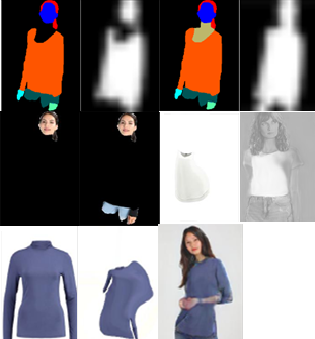
\includegraphics[height=8.5cm, scale=1]{figures/cpvtonissues.png}   % TODO
\caption{The issues in CP-VTON}
\label{fig:cpvtonissues}
\end{figure}


Firstly, the target try-on area is dependent upon current cloth shape. Especially, the neck area pixels are labeled as background and some body areas are occluded by hairs or accessories (Fig. 3 (a) left), which affects in cloth warping and blending. Secondly, all the unintended part, faces, bottom-clothes and legs have to be preserved in blending stage. But other parts except face and hair are missing in CP-VTON\cite{Wang2018TowardCI} human representation and generated at blending stage, which is all right for general synthesis application but not desirable in VTON application (Fig. 3 (b) left). Thirdly, the texture is often not vivid, which is due to the composition. Examining the original loss function of TON network, the term for the composition alpha mask are poorly formulated as simple regularization loss.   

\begin{equation}
L = c_1 | I_0-I_{GT} |+  c_2 L_{VGG}+c_3 |1-M_0 |        
\end{equation} 

Fourthly, since no label in the area of warped cloth is the same color as background, white colored clothes are confused and improperly processed in the blending stage (Fig. 3 (c))


Finally, GMM module using Spatial Transform Network\cite{JaderbergSZK15} with TPS (Thin Plate Spline)\cite{Bookstein1989PrincipalWT} deformation cannot handle strong 3D deformation due to the target pose and also generates artifacts because of the person representation inputs. For example, hands-up and folded arms.  Note that many errors in the warping stage are often hidden in the blending stage when the target clothes are single-colored, which can be expected in practical conditions 
%(Fig. 3 (d)).



%Especially note that the warped cloth are often too much different for desired shape. It is originated two facts. First the 3D deformation that any 2D deformation including non-rigid transform such as TPS is quite limited, especially any 2D deformation cannot handle when the two area in the original image are overlapped in the destination images. There for when the arms of long sleeved cloth occlude the main body, 2D warping cannot approximate the 3D deformation properly. Second, the deformation needs corresponding points  between the source nd target image. The cloth are extremely difficult object to find the corresponding points. The STN (spatial transform network)\cite{JaderbergSZK15} and SCM (shape context matching)\cite{BelongieMP02} cannot find the corresponding points when the target cloth and original cloth has different shapes. In conclusion, the 2D image based algorithm has serious limitation in the range of applications. It can apply to the mild posed target human only and simple short sleeved cloth, mainly because the inherent limitation of 2D deformation method including non-rigid ones, and the poor performance of matching algorithm.  To overcome this limitation, we consider to model the try-on cloth into 3D model and apply the 3D deformation

\begin{figure}
\centering
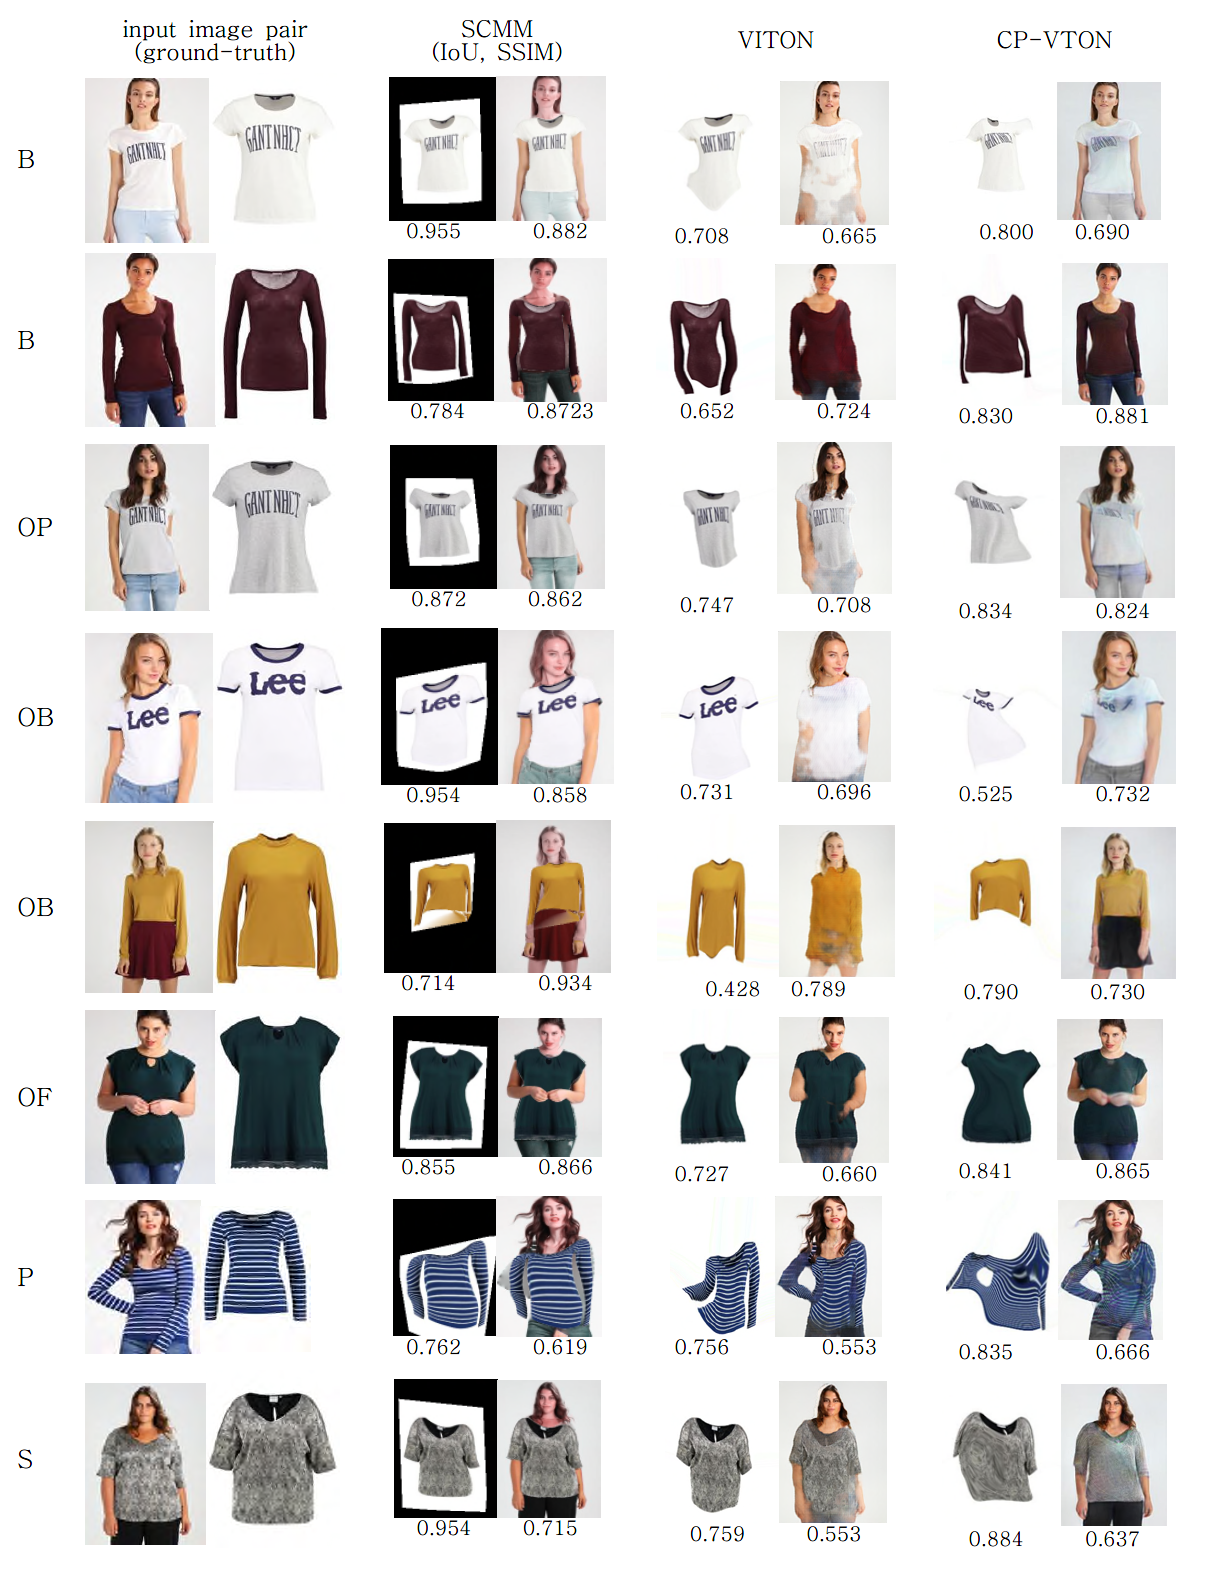
\includegraphics[height=13.5cm, scale=1]{figures/2dvton_same.png}   
\caption{Classified Evaluation of Image-based VTONs (same cloth re-try-on)}
\label{fig:2dvton_same}
\end{figure}

\begin{figure}
\centering
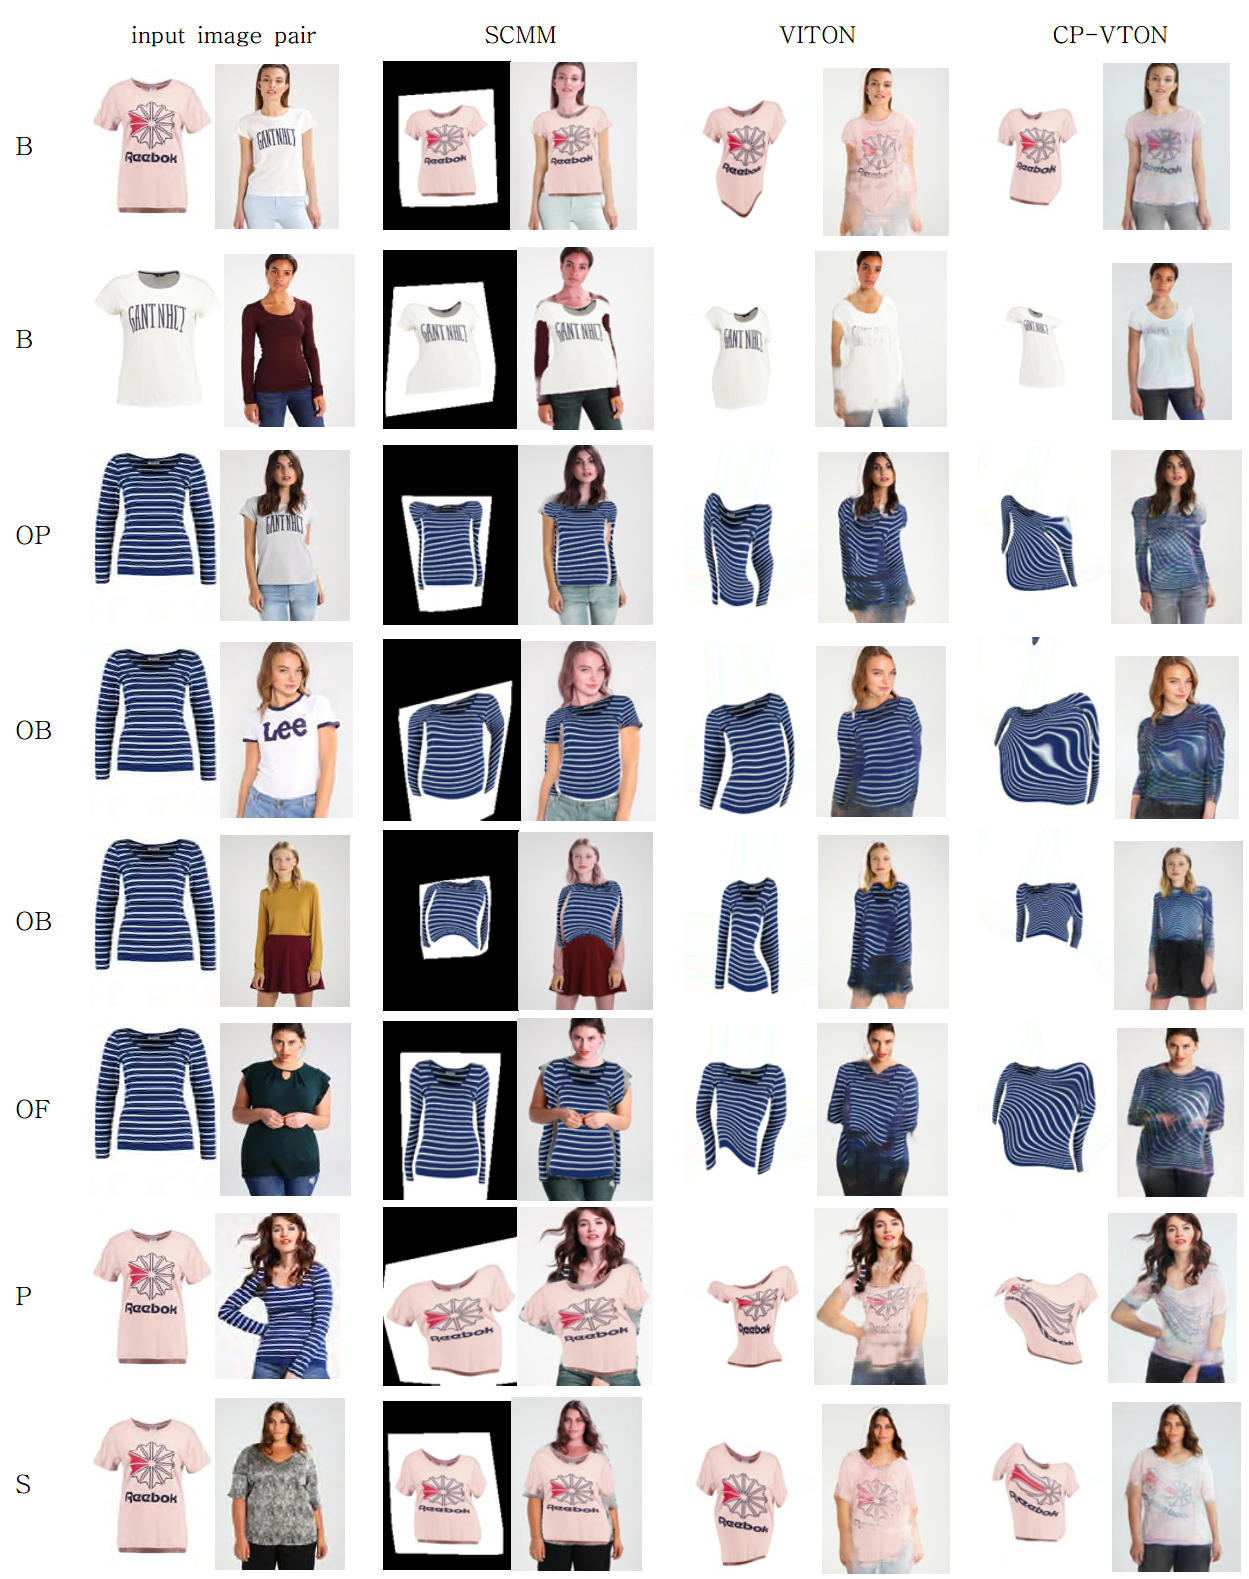
\includegraphics[height=13.5cm, scale=1]{figures/2dvton_diff.png}  %% TODO  
\caption{Classified Evaluation of Image-based VTONs (new cloth try-on)}
\label{fig:2dvton_diff}
\end{figure}
